\section{Package documentation}
\label{app:packagedoc}


The \texttt{SeaFire} package (SEmi-Analytical Feynman Integrals REsolution) can be imported in Mathematica using the command \texttt{Get[\dots]}, i.e. through \texttt{<< SeaFire.m}. Note that it has been developed and tested on \texttt{Mathematica 12.2}. 

Now we will go through all different functions and present their functionalities. 
\begin{itemize}
    \item \texttt{CurrentConfiguration[]}
    
    Returns the current configuration of the package. The configuration parameters can be modified using the function \texttt{UpdateConfiguration}.
    
    \item \texttt{UpdateConfiguration[NewConfig\_]}
    
    \texttt{NewConfig} must be a \texttt{List} whose elements are replacement rules \texttt{NameParameter -> NewValue}. The user has the possibility to modify these parameters
    
   \begin{table}[!h]
       \centering
       \begin{tabular}{|C{5 cm}|C{2 cm}| C{1.5 cm}|L{6 cm}|}
       \hline
        NameParameter & Value type & Default & Description \\
        \hline
        {\small\texttt{EpsilonOrder}} & \texttt{Integer} & 2 & {\small The maximum order in the dimensional regulator $\epsilon$ at which the system is expanded. Note that the minimum order is determined by the boundary conditions, that is if they contain a term $1/\epsilon^2$ the minimum order will be $-2$.} \\
        \hline
       {\small \texttt{ExpansionOrder}} & \texttt{Integrer} & 50 & {\small The maximum order in the kinematic variable at which the solution is expanded.}\\
        \hline
        {\small\texttt{InternalWorkingPrecision}} & \texttt{Integer} & 250 & {\small Specifies the number of digits that are used in internal calculations. If it is too high the execution will require more time and space, if it is too low we may face rounding errors.} \\
        \hline
        {\small\texttt{AvoidSingularities}} & \texttt{Bool} & \texttt{True} & {\small Specifies which method to use for transporting boundary conditions. \texttt{True} means that we are using the Taylor series approach described in section \ref{sec:taylor}. \texttt{False} means that we are using the Logarithmic series approach described in section \ref{sec:logarithmic}.}\\
        \hline
        {\small\texttt{RadiusOfConvergence}} & \texttt{Integer} & 2 & {\small It controls how fast we move at every expansion. In particular if \texttt{RadiusOfConvergence} is $n$, and the maximum radius of convergence of the solution is $d$, then the new point will be distant $d/n$ from the center of the series.}\\
        \hline
       \end{tabular}
   \end{table}
    
    \item \texttt{ReadFrom[FilePath\_]} 
    
    Utility function which reads from the specified path and return the content of the file. It is useful when the system of differential equations is particularly big and saved in a file.
    
    \item \texttt{SetSystemOfDifferentialEquation[System\_, BCs\_, MIs\_, Variables\_, PointBC\_, Param\_:\{\}]}
    
    Sets all the internal variables of the package and prepare the system of differential equations. It receives in input
    \begin{itemize}
        \item \texttt{System\_}: the system of differential equations. The equations must be ordered in a triangular form so that the first one is the simplest one and, at any particular order in $\epsilon$, inside the $n$-th equation does not appear the $n+1$-th master integrals. If there are multiple kinematics variables, one must pass firstly the system for the first variable, then for the second one and so on, where the order is specified in the \texttt{Variables\_} parameter.\\
        
        \textit{Example:}
        \begin{figure}[!h]
            \centering
            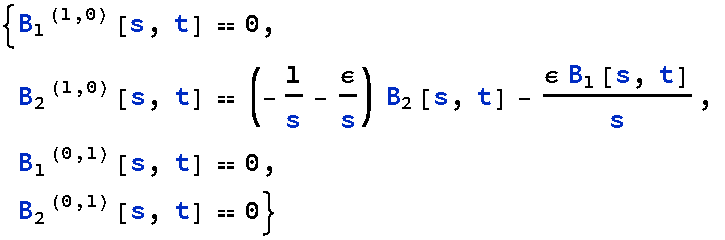
\includegraphics[scale=0.75]{Images/Code1.pdf}
        \end{figure}
        The first two equations refer to the kinematic variable \texttt{s}, while the last two to the kinematic variable \texttt{t}. The equations can be given expanded in $\epsilon$ or in a closed form in $\epsilon$.
        
        \item \texttt{BCs\_}: the boundary conditions the equations satisfy\\
        
        \textit{Example:}
        \begin{figure}[!h]
            \centering
            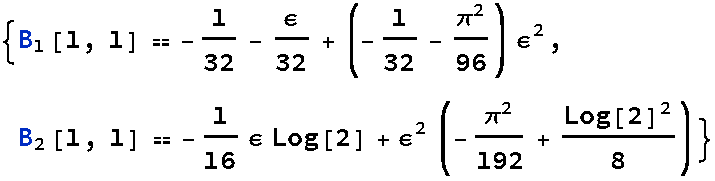
\includegraphics[scale=0.75]{Images/Code2.pdf}
        \end{figure}
        Also in this case they can be given in a closed form in $\epsilon$ or as a series. They can be exact or as floating numbers, in this case make sure that the precision of the boundary condition is greater than the \texttt{InternalWorkingPrecision}
        
        \item \texttt{MIs\_}: the list of master integrals, as they appear in the equations.\\
        
        \textit{Example:}
        \begin{figure}[!h]
            \centering
            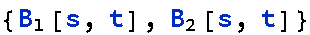
\includegraphics[scale=0.75]{Images/Code3.pdf}
        \end{figure}
        
        \item \texttt{Variables\_}: the list of variables appear in the equations, together with their Feynman prescriptions $\pm i \delta$\\
        
        \textit{Example:}
        \begin{figure}[!h]
            \centering
            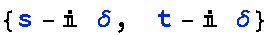
\includegraphics[scale=0.75]{Images/Code4.pdf}
        \end{figure}
        
        \item \texttt{PointBC\_}: the point in the phase-space in which the boundary conditions are imposed\\
        
        \textit{Example:}
        \begin{figure}[!h]
            \centering
            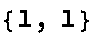
\includegraphics[scale=0.75]{Images/Code5.pdf}
        \end{figure}
        
        \item \texttt{Param\_}: this is an optional parameters, some equations might contain some external parameters, for example some masses \texttt{Mw}, \texttt{Mz}. Although the code works also with some external parameters inside the equations, because of how \texttt{Mathematica} works, it is extremely slower compared to a pure numerical system, for this reason it is always suggested to give numerical values to all parameters. This substitutions are performed before solving the system\\
        
        \textit{Example:}
        \begin{figure}[!h]
            \centering
            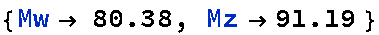
\includegraphics[scale=0.75]{Images/Code6.pdf}
        \end{figure}
    \end{itemize}
    
    \item \texttt{GetSystemOfDifferentialEquation[]} and\\ \texttt{GetSystemOfDifferentialEquationExpanded[]}
    
    Return the system of differential equations before and after it has been expanded in $\epsilon$. These functions can be used to check if everything has been set correctly.
    
    \item \texttt{SolveSystem[Variable\_]} 
    
    Solve the system of differential equations in the current point, that is where the boundary conditions are currently imposed.
    
    \item \texttt{GetPoint[]}
    
    Return the current point in which the boundary conditions are imposed.
    
    \item \texttt{TransportBoundaryConditions[Variable\_, Destination\_, Line\_:\{\}]}
    
    Transport the boundary conditions for the variable \texttt{Variable} from the current point to \texttt{Destination}, using the Taylor or logarithmic expansion accordingly to the \texttt{AvoidSingularities} configuration parameter. After transporting the boundary conditions to a certain point the current point is updated to \texttt{Destination}. The \texttt{Line} parameter is optional. If the user is not satisfied by the path automatically chosen by the package can use his own. The \texttt{Line} object must be created with \texttt{CreateLine}
    
    \item \texttt{CreateLine[Points\_]}
    
    Returns a line object that can be used in \texttt{TransportBoundaryConditions}\\
    
    \begin{figure}[!h]
        \centering
        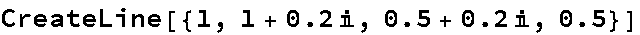
\includegraphics[scale=0.75]{Images/Code8.pdf}
    \end{figure}

    \item \texttt{Solution[]}
    
    Returns the series solution in the current point. The coefficients of the series are given with \texttt{InternalWorkingPrecision} digits. The result is given as a \texttt{List} and every MI as a Laurent series in $\epsilon$
    \begin{figure}[!h]
        \centering
        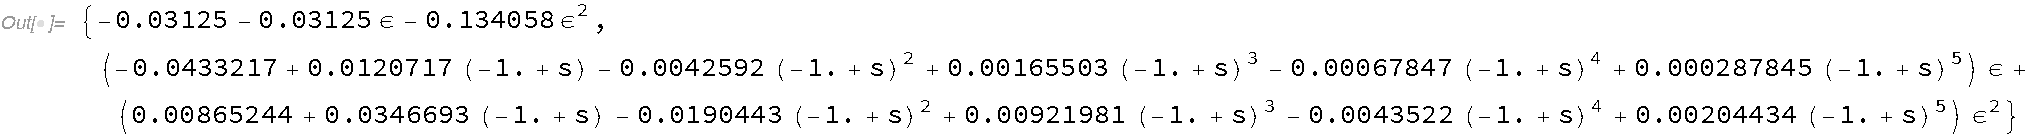
\includegraphics[width=\textwidth]{Images/Code7.pdf}
    \end{figure}
    
    % \item \texttt{PerformMobiusTransformation[Variable\_]}
    
    % Perform a Möbius transformation with respect to \texttt{Variable}, note that \texttt{Variable} must the last variable we solved the system with respect to.  
    
    % \item \texttt{GetSolutionExpanded[]}
    
    % Returns the solution after performing the Möbius transformation.
    
    \item {\small\texttt{CreateGraph[MI\_, EpsOrder\_, Left\_, Right\_, OtherFunctions\_:\{\}]}}
    
    Draws a \texttt{ReImPlot} of the solution of order \texttt{EpsOrder} for the master \texttt{MI}. The graph runs from \texttt{Left} to \texttt{Right}. 
    %The option \texttt{Mobius} can be used to control if the solution to be plotted is the one after Möbius transformation or not. 
    The argument \texttt{OtherFunctions} may contains other functions to be plotted in the same graph.
\end{itemize}






